\documentclass{article}
\usepackage{graphicx} % Required for inserting images
\usepackage{natbib}
\usepackage{amsmath}
\usepackage{url} 
\usepackage[hidelinks]{hyperref}
\usepackage[T1]{fontenc}
\usepackage{mathpazo,euler}
\usepackage[scaled=0.9]{DejaVuSans}
\usepackage[utf8]{inputenc}
\usepackage{listings}
\usepackage{tabularx}
\usepackage{amsfonts}
\usepackage{booktabs}
\usepackage{siunitx}
\usepackage{geometry}

\geometry{margin=1in}
\lstset{basicstyle=\ttfamily}
\bibliographystyle{abbrvnat}
\setcitestyle{authoryear,open={(},close={)}} % Citation-related commands

%\title{First Year Paper}
\title{First Year Paper} % Add your subtitle here

%\subtitle(Advisor: Moisés Expósito Alonso)
\author{Tatiana Bellagio \\ Advisor: Moisés Expósito Alonso}
\date{November 2023}
\begin{document}

\maketitle

\tableofcontents
\newpage % Starts a new page after the table of contents

\section{Introduction}
\subsection{Shift, Adapt or Perish}
When species' populations face environmental changes they can follow one of three available options: shift their geographical distribution to track suitable environments, adapt to the new imposed conditions, or face death or even extinction. Adaptation refers to the process by which a population becomes better suited to its environment through changes in its genetic makeup. In the face of anthropogenic-generated rapid environmental changes, understanding the dynamics of evolution over short time scales becomes more important than ever \citep{Waldvogel2020-dh}.

\subsection{But what is rapid evolution?}
Evolution has been historically thought as a slow and gradual process occurring over extensive timescales, often spanning thousands to millions of years. However, genetically based rapid phenotypic changes have been shown to be pervasive in nature. The famous peppered moth \citep{Cook2013-bs}, insecticide resistance in Drosophila \citep{Daborn2002-is}, color of field mice \citep{Vignieri2010-if}, beak size in Darwin’s finches \citep{Grant2008-uc}, guppies in Trinidad \citep{Kemp2009-ji}, and Anolis lizards \citep{Losos2009-vq} are some examples.

Rapid evolution can be defined based on the number of generations in which a change can be foreseen but also as the convergence of ecological and evolutionary times \citep{Hairston2005-qo}. This last statement, is of particular importance and highlights rapid evolution as one of the more applied domains within evolutionary studies. This immediacy is crucial in addressing urgent ecological and conservation issues, where understanding and predicting the pace and direction of evolutionary changes can inform conservation strategies and management practices. 

\subsection{Trait architecture and adaptation}
The discussion about what type of genetic diversity disposition and distribution across the genome can fuel adaptation comes a long way. Since Darwin (Darwin 1859) and Huxley (Huxley 1860) discussions about whether the nature of adaptation is characterized by incremental, subtle variations in many loci or by significant, abrupt changes on only a few of them. Compelling evidence shows that both cases are true, there is considerable heterogeneity in architectures among adaptive traits \citep{Orr1992-xj, Orr1998-pr}. 

The next question that arises from this is what is the implication of different genetic architecture on the adaptation process? Different works have explored thee evolutionary dynamics of different trait architectures \citep{Hayward2021-ji, Stetter2018-st, Thornton2019-ww}. Nevertheless, all these works follow and old view, spanning long time periods and extending over hundred or thousands of generations to determine the outcome. Also, most cases focus on genetic variation entering the population through new mutations, while in short periods of times populations will most likely dependent solely on standing genetic variation. Overall, the implication of different trait genetic architectures from standing genetic variation on the dynamics of rapid evolution has not been yet explored. 

\subsection{Detecting adaptive loci after rapid evolution}
The genomic footprints of an adaptation process can be one of three types: hard sweeps, soft sweeps, and polygenic signals. These patterns will depend on the genetic architecture of the original adaptive trait. Historically, most selection scans have focused on detecting hard sweep (cite) because they align with a classical population genetic view and because of the more discernible genetic patterns they leave,a decrease in diversity at the selected region compare to rest of the genome. More than a decade ago, Pritchard and Di Rienzo already highlighted that the vision of adaptation that proceeds by selective sweeps at key loci is too limited, and the more polygenic view coming from the field of quantitative genetics should be incorporated \citep{Pritchard2010-bv}. After this, more efforts have been focus on detecting polygenic signal of adaptation \citep{Berg2014-zl}.

Mainly under polygenic adaptation, the mere genomic signals might not be powerful enough to detect adaptive loci, but power could be earned by incorporating the actual selective pressures on the equation. Focusing on climatic selective pressures, if we assume than certain loci are responsable for climate adaptation, we would expect to find a linear relationship between an environmental gradient and the allele frequencies of populations situated across that gradient. This approach has been used to developed different pieces of software including LFMM \citep{Frichot2013-mg}, Bayenv \citep{Gunther2013-fw}, and an expanded implementation of bayenv core model in Baypass \citep{Gautier2015-lp}.

\subsection{How can we study rapid evolutionary dynamics? }
\subsubsection{Simulations}
In nature, selection forces are pervasive, and populations are simultaneosuly imposed to selective pressure acting on multiple traits spannign a range of genetic architectures, making it difficult to disentangle particular relationships. In this sense,  a way of disecting the complexity imposed in the real world, is through simulations. Forward in time individual based genetic simulations represent a powerful tool that allow the manipulation of known relevant parameters to get a deep understanding of key factors influencing evolutionary dynamics and outcomes. Simulations can allow us to not only understand how key parameters can affect the evolutionary processes, but also replicate real experiments to build a null hypothesis and build expected results about the real world.  With this in mind, they also allow us to explore the best statistical approaches to use for our data and detect the signals we are looking for. 

\subsubsection{Experiments}
On one hand, Evolve and Resequence experiments (E\&R) \citep{Schlotterer2015-yz}, are a methodology usedto study the genetic basis of adaptation and evolutionary processes. They combine the principles of experimental evolution with sequencing techniques and are based on  applying selective pressures in controlled environments and then sequencing the genomes of evolving populations over time. E\&R
are particularly well-suited to study rapid evolution because they allow to observe evolutionary changes over relatively short periods. Some succesful examples inlcude \citep{Bergland2014-ud, Kapun2021-cd, Rudman2022-uc}.  , bergland being able to to describe allele frequencies shifting seasonally in Drosophila populations. 

On the other hand, one of the most used experimental designs to find signal(E\&R)s of local adaptation are common garden. Common gardens consist of growing individuals from different populations in the same set of controlled environments. By controlling the environment, any differences observed among populations in are likely due to genetic variation. Some succesful examples are \citep{Exposito-Alonso2019-hs, Lepais2014-za}.

A combined approach of (E\&R) and common garden experiments could be unusually powerful to identify the genomic regions responsable for climatic adaptation and to better understand rapid evolutionary dynamics. With this in mind, a multi generation and globally distributed common garden experiments was conducted, where 34 founder \textit{Arabidopsis thaliana} populations where planted and resequence over 4 years (\url{http://grene-net.org/})

\subsection{What is new?}
Since the relationship between different genetic architectures and the dynamics of rapid evolution has not been yet explores, we decided to conduct a set of simulations to achieve this. Also, inspired by the power of studying rapid evolution across a gradient of environments, we decided to inspire our simulations on a real experiment, Grene-Net, so that the outcomes would also be useful as a ground truth for benchmarking and setting realistic expectations regarding the detectability of adaptive loci across various genetic architectures in the real data. 

Hence, this project aims to answer two main questions: 
\begin{itemize}
    \item Are rapid evolutionary dynamic different when the adaptive trait has a range of different genetic architectures? 
    \item Can we then detect the loci encoding the adaptive traits acrros a gradient after a rapid evolution process?
\end{itemize}

\section{Methods}
\subsection{Simulations}

Simulation software
We used SLiM \citep{Haller2019-oj} for running a total of 189000 independent forward in time genetic simulations based on all combination of parameters plus replicated.  Each simulation represents a single population monitored for 10 generations. SLiM uniquely allowed us to have flexibility to simulate all the parameters below indicated, model specifics to \textit{A. thaliana} biology and work with tree sequences structures to achieve our goals in a computational efficient fashon. 

\subsubsection{Genetic diversity}
Because standing genetic variation is the subtract of rapid evolutionary changes rather than de-novo introduced genetic diversity via mutations, and to make our simulations more realistic we decided to work with real standing genetic variation. Since we were also interested in using this set of simulations as ground truth for the Grene-Net project we decided to use the genetic information from its founder populations. The founder population for all simulations consisted of a pool of 2310 individuals representing 231 different ecotypes coming from divergent climates across the world (full table of ecotypes in suplementary information), making it a highly diverse pool of individuals. 

\subsubsection{Trait genetic architecture}
We decided to model only one trait in which selection would act. We defined the trait genetic architecture based on three key parameters: polygenictiy, initial allele frequency and effect size. Polygenicity is defined as the total number of loci contributing to the trait value, and we calculated traits with 7 different levels for it. \ref{simulation_parameters_table}). We also built traits which encoding loci had 6 different ranges of initial allele frequency (Table \ref{simulation_parameters_table}). Finally the the effect size of each contributing loci was drawn from \( \sim N(0, 2) \) for all simulations

\subsubsection{Genetic value, heritability, environmental variance, and phenotype}

We used the additive genetic model for calculating the genetic value of each individual, such that \\ $A_n=\sum a_i$, where $A_n$ is the genetic value of the individual $n$ and \( a_i \) represents the effect size of the \( i \)-th contributing locus. We simulated 5 different levels of heritability for the trait (Table \ref{simulation_parameters_table}). For each simulation, using the breeders equation, we calculated:
\[
VE = \frac{VA - h^2 \cdot VA}{h^2}
\]
where \( VE \) is the environmental variance, \( VA \) represents the genetic variance from the given population \( VA = \text{Var}\left(\sum A_n\right) \), and \( h^2 \) is the heritability value for the given simulation. Once we had the value of \( VE \) we drew random samples of environmental noise (\( en \)) for each individual \( en_n \sim N(0, VE) \)to then calculate the phenotypic trait value of each individual by \( y_n = A_n+ en_n \). For each simulation we obtain the standard deviation and mean of the initial population to then use those values to standarize the phenotypes each generation before the fitness calculation.

\subsubsection{Selection function and fitness}
Each individual n was subjected to stabilizing selection based on their phenotypic value with the formula:
\[
\text{Fitness}_\text{n} = \exp\left(-0.5 \times \frac{(\text{Phenotype}_\text{n} - {\text{Optimum phenotype}_\text{k}})^2}{\text{V}_\text{s}}\right)
\]
Were $\text{Optimum phenotype}_\text{k}$ refers to the optimum phenotype at the k environment and $\text{V}_\text{s}$ represent the strength of stabilizing selection. We simulated 4 different levels of it (Table \ref{simulation_parameters_table}). Finally,  $\text{Fitness}_\text{n}$ would serve as a probability of survival of the individual n to the next generation. The different strength of selection are depicted in Fig. \ref{fig:selection_strength}. 

\subsubsection{Population density control}
In all simulations the starting population size was 2310 individuals, but after the first selection episode, and on every cycle, if the population reached a size larger than 900 individuals, we would randomly subtract individuals to keep it at 900. This is based on the observations of the real experiment, where the biggest populations only reached a maximum of 900 individuals. 

\subsubsection{Environmental gradient}
We simulated 9 different environments (Table \ref{simulation_parameters_table}), each one defined by its distance in standard deviations from the initial phenotype mean. Environment 0 would have 0 standard deviations from the initial phenotype mean, so that individuals situated exactly in the initial mean phenotype value would have a fitness of 1. The different simulated environments are depicted in Fig. \ref{fig:selection_strength}. 

\subsubsection{Specifics to \textit{A. thaliana} biology}
Because one of our main focus was to simulate the evolutionary dynamics of the Grene-net project we decided to add some specifics of \textit{A. thaliana} biology, besides its populations genetic diversity. Firstly, we used \textit{A. thaliana} mean recombination rate across the genome of $3 \times 10^{-6}$. Since \textit{A. thaliana} is an annual plant, we simulated non-overlapping generations, and all progenitors would perish in each cycle. Finally, we decided to use strict information about \textit{A. thaliana} reproductive strategies, simulating a 97\% slefing rate, 3\% outcrossing rate, and a litter size taken from $\sim Poisson(7.247)$. This value was informed from actual common garden experiments (cite Laura?). 

\subsubsection{Data Structure}
Since we wanted to simulate the genetic diversity on its fullest to be able to accurately benchmark the softwares to detect the causal loci down the line, we decided to make use of the tree sequence structures for the simulations \url{https://github.com/tskit-dev/pyslim}. For this, we took the initial population VCF file with the full genetic information and converted into a tree sequence structure. After defining the genetic architecture of each simulation and randomly choosing the contributing loci, we kept only those mutations in the tree sequence structure and subtracted and separately saved all other neutral mutations, making the tree lighter and faster to run on SLiM. For each simulation, after it finished we overlaid the previously removed neutral mutations on the output tree, obtaining as the final result the tree sequence with neutral and adaptive mutations on its fullest. 

\subsubsection{Data Collection}
For each simulation on each generation we collected key parameters including: fitness mean, fitness variance, population size, phenotype mean and phenotype variance. 

\subsubsection{Reproducibility}
To ensure reproducibility and trackability of all analysis, we developed a snakemake \citep{Molder2021-ho} pipeline starting with the initial VCF file from the founder population and finalizing with the benchmarking of all softwares. If desired, the pipeline could be rerun on its fullest. The code for the entire pipeline is available at \url{https://github.com/Tatianabellagio/slim_grenenet}.

As observed in \ref{fig:slopes_lr} 
\subsection{Benchmarking}

We benchmark 5 different softwares, that can be clasified in two main categories. The first category of softwares comes from 

LMM (Linear Mixed Model) Approach 

LFMM (Latent Factors Mixed Model) Approach

Bayenv + Bypass Approach 

GWAS (Genome Wide Association Study) Approach 

HapFM (Haplotype based Fine Mapping) Approach 

\section{Results}

\subsection{Survivalship vs each simulation parameter}

In order to understand the relationship between each of the parameters independently of all others used in our simulation and the population's survivalship, we decided to run logistic regressions for each of the parameteres, keeping all the other parameters constant. Survivalship was meassured as the percentages of populations that survived to the 10th generation. For this analysis, we report the slope fitted for the logistic regression divided by the estimated error. A positive slope would indicate a positive relationship between survivalship and an increment in the evaluated parameters. We only considered slopes which p value was less than 0.05. 

As observed in \ref{fig:slopes_lr} certain parameters had expected behaviour, such is the case of the distance to the new optimum from the initial population mean, always showing a negative slope for any combination of the other parameters. This aligns with an expected behaviour, where, the further the new optimum is from the initial mean of the population, the less survivalship the populations are going to encounter. The opposite relationship is observed in the case fo the selection strength, which is also expected. For any combination of parameters an incresease in the variance value for the calculation of the fitness function leads to an increase suvivalship of the population. In the case of heritability, most values are above 0, indicating that most of the times an increase in the heritability value would leas to an increase survivalship. For the the polygenicity an inital allele frecuency of the contributing loci the slope values are disperse across positive and negative values, so we decided to explore this further. 

First, in \ref{fig:survivalship_forpoly} we can observe the proportion of populations that survived for the combination of each parameters but polygenicity. Then, in \ref{fig:polydependence} the layout of parameters is the same, but now we instead of suvivalship the color scheme represents the slope of each logistic regression run between  survivalship and polygenicity for each combination of parameters. In \ref{fig:poly_survival_transparency} we overalp \ref{fig:survivalship_forpoly} on \ref{fig:polydependence} and now survivalship is represented as trasnparency. This hihglights the a clear diagonal pattern of positive slopes when populations have an intermediate survivalship. This supports the hypothesis that populations wiht a more polygenic trait are favored at the 'edge' of the ditribution. When selection is not  very strong or the population is close the new optimum (lower corner) the polygenicity is not a limiting factor, neither when selection is very strong or the populations are very far away from the new optimum (upper corner), since most population die anyways (as shown in \ref{fig:survivalship_forpoly}). Finally, we see some negative relationships between survivalship and polygenicity mainly at very low allele frequency and when the new optimum is far away, this might be a side effect from the phenotypes standarization. As shown in \ref{fig:phenotypes_initial} the phenotypes distribution in the monogenic architecture with low allele frequency (0-5\%) has a peak at the tails, wich is an artifact of the phenotype standarization. 

Also, we were interested in why heritability did not show aways a positive reltaionship with survivalship in \ref{fig:slopes_lr} as would be expected, since heritability is the evolutioary memory of evolution and we would expect that heritability would be necessary fro population to evolve towards the new optimum. To explore this, we first show the relationship between survivalship and all the other parameters but heritability \ref{fig:h2_survival_transparency} and then with this same 


\begin{table}
\centering
\begin{tabularx}{\textwidth}[t]{XX} \toprule
{Parameter} & {Values} \\ \midrule
{Number of contributing loci to the trait} & {[1, 5, 20, 50, 100, 200]} \\ \midrule
{Initial frequency of contributing loci} & {[0-0.05, 0.1-0.2, 0.2-0.4, 0.4-0.6, 0.6-0.8, 0.8-1]}\\ \midrule
{Trait heritability} & {[0.1, 0.3, 0.5, 0.7, 0.9]} \\ \midrule
{Distance to new optima (standard deviations from initial phenotypes mean value)} & {[0, 1, 2, 3, 4]}\\ \midrule
{Variance of stabilizing selection} & {[0.1, 0.01, 0.001, 0.0001]} \\ \bottomrule
\end{tabularx}
\caption{Simulation parameters table}
\label{simulation_parameters_table}
\end{table}

\begin{figure}[b]
    \centering
    \includegraphics[width=1\textwidth]{figures/parameters.pdf}
    \caption{Caption of the figure.}
    \label{fig:parameters}
\end{figure}

\begin{figure}[b]
    \centering
    \includegraphics[width=1\textwidth]{figures/phenotypes_initial-3.pdf}
    \caption{Caption of the figure.}
    \label{fig:phenotypes_initial}
\end{figure}

\begin{figure}[b]
    \centering
    \includegraphics[width=1\textwidth]{figures/phenotypes_initial_onlymonogenic-2.pdf}
    \caption{Caption of the figure.}
    \label{fig:phenotypes_initial_mono}
\end{figure}

\begin{figure}[b]
    \centering
    \includegraphics[width=1\textwidth]{figures/slopes_lr.pdf}
    \caption{Caption of the figure.}
    \label{fig:slopes_lr}
\end{figure}

\begin{figure}[b]
    \centering
    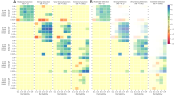
\includegraphics[width=1\textwidth]{figures/poly_panel_figure_2plots.pdf}
    \caption{Caption of the figure.}
    \label{fig:poly_panel_figure}
\end{figure}

\begin{figure}[b]
    \centering
    \includegraphics[width=1\textwidth]{figures/h2_panel_figure_2plots.pdf}
    \caption{Caption of the figure.}
    \label{fig:h2_panel_figure}
\end{figure}


\begin{figure}[b]
    \centering
    \includegraphics[width=1\textwidth]{figures/survivalship_forpoly-1.pdf}
    \caption{Caption of the figure.}
    \label{fig:survivalship_forpoly}
\end{figure}



\begin{figure}[b]
    \centering
    \includegraphics[width=1\textwidth]{figures/survivalshipforh2-1.pdf}
    \caption{Caption of the figure.}
    \label{fig:survivalshipforh2}
\end{figure}

\section{Discussion}

the trait. In the opposite case of mostly large effects, rapid fixations (leading to selective sweeps) may produce fast phenotypic responses. In the examples of fast adaptation mentioned in the Introduction, both of these extremes and combinations thereof have occurred.(Jain and Stephan 2017)
More generally, our analysis also provides some new insights into the question whether selective fixations (and thus sweeps) occur at QTL. While Chevin and Hospital (2008) predicted that the probability of selective sweeps is extremely low at QTL (based on a model with one major locus and infinitely many minor loci), others have found sweeps at appreciable frequencies using simulations of various multi-locus models (Pavlidis et al. 2012; Wollstein and Stephan 2014). The prediction of Chevin and Hospital is consistent with our study for mostly small-effect loci and small shifts in the phenotypic optimum. (Jain and Stephan 2017)



\bibliography{paperpile} % Bibliography

\end{document}
